% !TeX spellcheck = en_US
\cleardoublepage\phantomsection\addcontentsline{toc}{section}{\protect\numberline{} {} {} {} {}Elixir of Life}
\addscenariosection[subsection]{1}{Rampart coop Campaign $-$ Elixir of Life}{1. Graduation Exercise}{\images/gelu.png}

\begin{multicols*}{2}

\textbf{Author:} Tm335

\textit{Gelu is the youngest individual to ever graduate from the Forest Guard.
  He must pass one final test and then he will enter service under Lord Falorel: assemble the pieces to the Elixir of Life so the Deyjan lords can't destroy the precious combination artifact.
}

\textit{The Forest Guard is Erathia’s eyes and ears.
  We go where we are needed most and that is usually places difficult for traditional fighting forces to reach.
  We are shadows of the forest that see all and bring silent death with a single, unseen bowshot.
  You have done well in your training, Gelu, but now has come the time to take the final test.
  A small valley near Gaia's Crest will be the site of this trial.
  Clear the region of all the enemies to earn your place among the ranks of the Forest Guard.
  Good luck.
}

\subsection*{\MakeUppercase{Scenario Length}}

This Scenario plays out over 13 Rounds.

\subsection*{\MakeUppercase{Player Setup}}

\textbf{Player Count:} 2

\textbf{Faction:} Rampart

\textbf{Faction Hero:} Gelu (player 1), and Mephala or Clancy (player 2)

\textbf{Starting Resources:} 15 \svg{gold}, 3 \svg{building_materials}, 1 \svg{valuables}

\textbf{Starting Income:} 10 \svg{gold}, 0 \svg{building_materials}, 0 \svg{valuables}

\textbf{Starting Units:} A Few Centaurs, a Few Dwarves, a Pack of Elves, a Few Pegasi

\textbf{Town Buildings:} \bronze\ Dwelling, \silver\ Dwelling, Mystic Pond

\columnbreak
\textbf{Bonus:}
\begin{itemize}
  \item One player adds the Speculum Artifact to their hand.
  \item One player gains 1 \svg{experience}.
\end{itemize}

\subsection*{\MakeUppercase{Coop Play Rules}}

In addition to the Cooperative Mode rules (see page 11, ``Cooperative Mode'' in the Core Mission Book), reference the attached \pagelink{Coop Campaign Rules}{Coop Campaign Rules} specific to this campaign.

\subsection*{\MakeUppercase{AI Hero Setup}}

\textbf{Faction:} Necropolis, Inferno, Dungeon

Refer to the \hyperlink{Elixir of Life AI}{table below the map layout} for detailed information about Units and AI Decks.

\subsection*{\MakeUppercase{Map Setup}}

Take the following Map Tiles and arrange them as shown in the Scenario map layout:

\textbf{4 × Starting (I) Map Tile}
\begin{itemize}
  \item 1 × Rampart (S4)
  \item 1 × Inferno (S6)
  \item 1 × Necropolis (S1)
  \item 1 × Dungeon (S2)
\end{itemize}

\textbf{4 × Far (II--III) Map Tile}
\begin{itemize}
  \item 4 × Castle/Rampart (F10 and choose 3 from: \#F4, F6, \#F8, F9, F11, F12)
\end{itemize}

\textbf{4 × Near (IV--V) Map Tile}
\begin{itemize}
  \item 2 × Castle/Rampart (choose 2 from: \#N3, N6, N8)
  \item 1 × Castle (N3)
  \item 1 × Dungeon (N5)
\end{itemize}

\subsection*{\MakeUppercase{Heroes Placement}}

Place Necropolis, Inferno, and Dungeon Heroes in their respective Faction Towns.
Place Gelu on the center Field of the Rampart S4 Starting Map Tile.
Place either Mephala or Clancy on an empty Field of the F10 Map Tile.
Place the Pack of Medusas on the Far Map Tile as indicated in the Scenario map layout.

\subsection*{\MakeUppercase{Victory Conditions}}

Defeat and capture all enemy Faction Towns.

\subsection*{\MakeUppercase{Defeat Conditions}}

You lose if any of the following occur:
\begin{itemize}
  \item Gelu is defeated in a Combat encounter.
  \item You fail to capture the Necropolis and Inferno Faction Towns in a single Round.
  \item You fail to capture all Enemy Faction Towns before the end of Round 13.
\end{itemize}

\subsection*{\MakeUppercase{Timed Events}}

\textbf{\nth{1} Round:}
\begin{itemize}
  \item Read: ``Exercise starts'' section.
  \end{itemize}

\textbf{Discovering the Tile with Medusas:}
\begin{itemize}
  \item Read: ``A quiet trail'' section.
\end{itemize}

\textbf{\nth{5} Round:}
\begin{itemize}
  \item Read: ``The raiders'' section.
\end{itemize}

\textbf{Entering the Field with Pandora's Box:}
\begin{itemize}
  \item Read: ``Pandora's Box'' section.
\end{itemize}

\textbf{\mbox{\nth{9} and all the following Resource Rounds:}}
\begin{itemize}
  \item Read ``Continued raids'' section.
\end{itemize}

\textbf{When you complete the Scenario:}
\begin{itemize}
  \item Read: ``Congratulations! You have passed the Trial! Victory is yours!''
\end{itemize}

\columnbreak

\subsection*{\MakeUppercase{Additional Rules}}

During this Scenario:

\begin{itemize}
    \item Gelu cannot surrender.
      Player 2 can surrender.
      If player 2 is defeated in Combat, lose 5 \svg{gold} and both Heroes gain a \svg{morale_negative} token.
      Player 2 Hero is then placed in any Town or Settlement you control, or on a Field adjacent to Gelu.
    \item Your Heroes do not gain Experience past Level 5.
    \item You cannot recruit a Secondary Hero.
    \item Enemy Heroes stay within their Towns. They do not move.
    \item At the Dragon Utopia location, your Hero fights the Gold Dragons Army.
    \item Gain 1 \svg{valuables} when you defeat an Enemy Hero Army.
    \item \textbf{The Obelisks at N3 and N5 are Two-Way Monoliths.}
      Entering one of these Fields transports your Hero to the other Field. \textbf{The Obelisks function only if both Necropolis and Inferno Faction Towns have been captured.}
    \item \textbf{Inferno Town contains a one-way Castle Gate} that will allow the Player to transport themselves to the Obelisk at N3. It works only if the N3 Obelisk was flagged.
  \item \textbf{Necropolis and Inferno Towns:} The Necropolis and Inferno Towns (on S1 and S6) MUST be attacked and captured in the same Round.
    The Round is determined by when either Map Tile S1 or S6 is entered.
    If this coordinated attack fails, Gelu will lose his cover, and all Enemy Towns will call for immediate reinforcements.
    Gelu is then defeated.
\end{itemize}

\end{multicols*}

\begin{minipage}{\textwidth}
  \vspace{-3em}
  \begin{tikzpicture}[remember picture]
    \node(map)[anchor=center] at (9, -4.5) {
      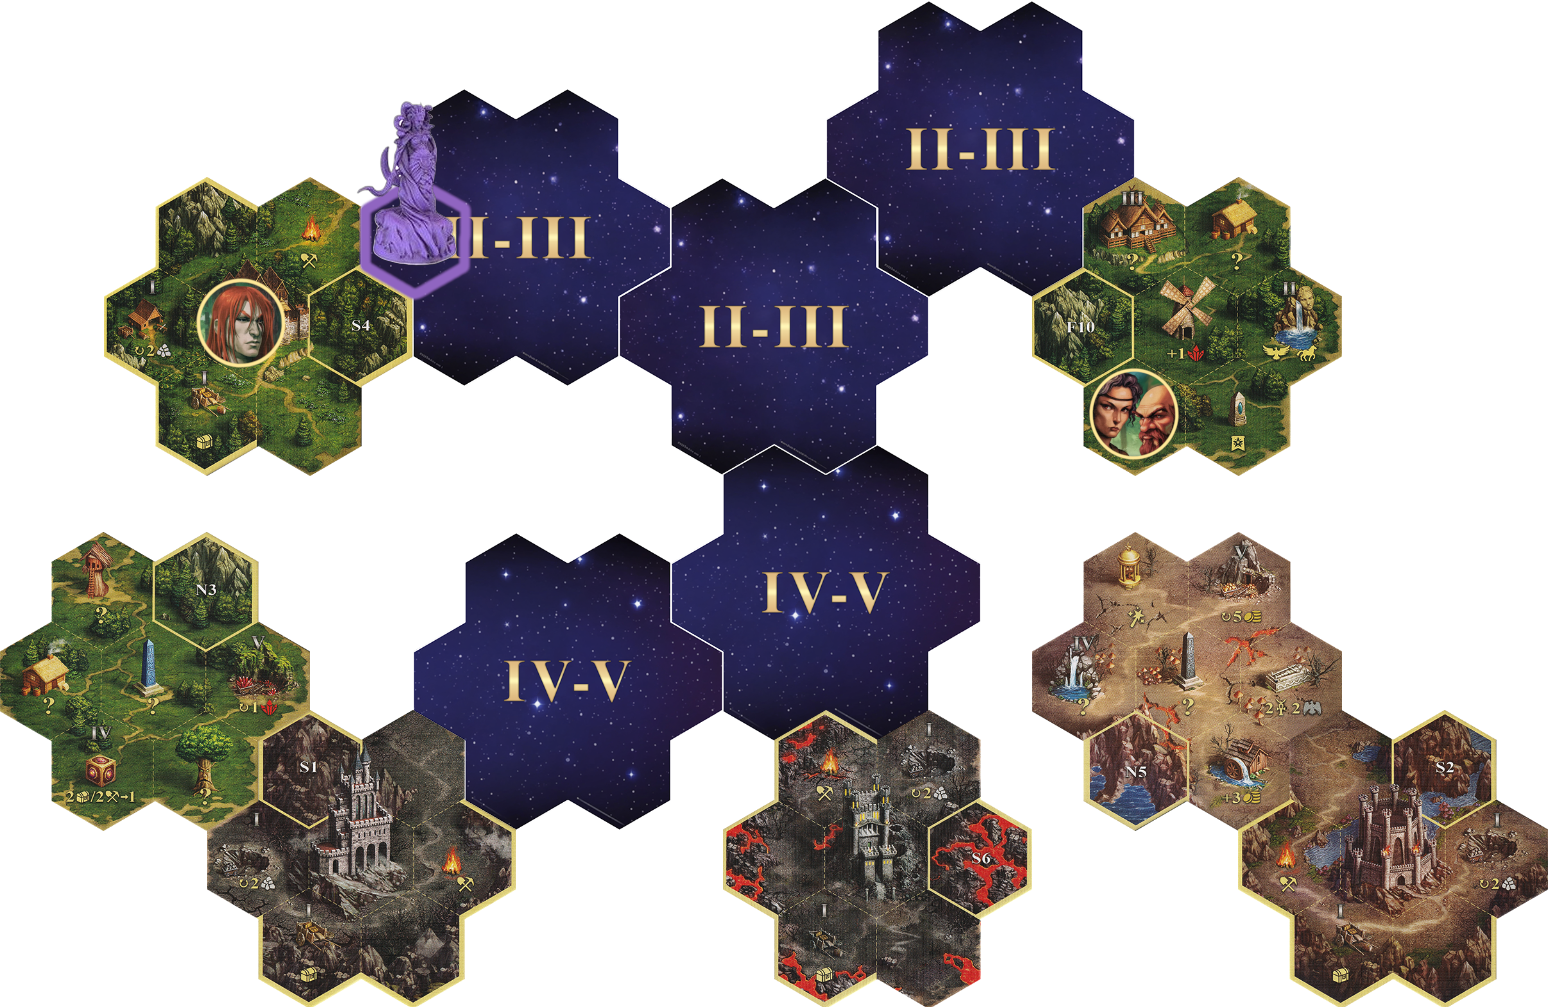
\includegraphics[width=\textwidth]{\maps/rampart_graduation_exercise.png}
    };
    \node at (1.3,-1.4) {\large{{\textbf{\textcolor{darkcandyapplered}{S4}}}}};
    \node at (3.3,0.5) {\large{{\textbf{\textcolor{darkcandyapplered}{Pack of}}}}};
    \node at (3.3,0) {\large{{\textbf{\textcolor{darkcandyapplered}{Medusas}}}}};
    \node at (15.6, -1.4) {\large{{\textbf{\textcolor{darkcandyapplered}{F10}}}}};
    \node at (3.5, -5.5) {\large{{\textbf{\textcolor{darkcandyapplered}{N3}}}}};
    \node at (15.6, -5.5) {\large{{\textbf{\textcolor{darkcandyapplered}{N5}}}}};
    \node at (5.9, -9.7) {\large{{\textbf{\textcolor{darkcandyapplered}{S1}}}}};
    \node at (14.5, -9.7) {\large{{\textbf{\textcolor{darkcandyapplered}{S2}}}}};
    \node at (11.9, -9.7) {\large{{\textbf{\textcolor{darkcandyapplered}{S6}}}}};
  \end{tikzpicture}
\end{minipage}

\vspace*{\fill}

\begin{table*}[!hb]
  \hypertarget{Elixir of Life AI}{}
  \hommtable[]{24}{
    \centering
    \medskip
    \textbf{AI Hero Setup}\\
    \medskip
    \begin{tabularx}{0.95\linewidth}{>{\centering}p{0.15\linewidth}>{\raggedright\arraybackslash}X>{\centering\arraybackslash}X>{\centering\arraybackslash}X}
      \darkcell{Faction} & \darkcell{Units} & \darkcell{AI Deck} & \darkcell{Spells} \\
      \darkcell[2.8]{Necropolis}
      & \lightcell[2.8]{Pack of Zombies\\Pack of Wraiths\\Pack of Liches\\Few Dread Knights\\Walls and Gate}
      & \lightcell[2.8]{1~×~Might \svg{might-yellow} Card\\3~×~Magic \svg{magic-yellow} Card}
      & \lightcell[2.8]{1~×~Resurrection\\1~×~Haste\\1~×~Weakness} \\
      \darkcell[2.8]{Inferno}
      & \lightcell[2.8]{Pack of Magogs\\Pack of Cerberi\\Pack of Pit Lords\\Few Efreet\\Walls and Gate}
      & \lightcell[2.8]{3~×~Might \svg{might-yellow} Card\\1~×~Magic \svg{magic-yellow} Card}
      & \lightcell[2.8]{1~×~Fireball} \\
      \darkcell[3.2]{Dungeon}
      & \lightcell[3.2]{Pack of Harpies\\Pack of Evil Eyes\\Pack of Medusas\\Few Manticores\\Few Black Dragons\\Walls and Gate}
      & \lightcell[3.2]{3~×~Might \svg{might-yellow} Card\\3~×~Magic \svg{magic-yellow} Card}
      & \lightcell[3.2]{1~×~Magic Arrow\\1~×~Slow\\1~×~Sorrow} \\
    \end{tabularx}
  }
\end{table*}

\vspace*{-1.5em}

\pagebreak

\begin{multicols*}{2}

\subsection*{\MakeUppercase{The Story}}

\textbf{Exercise starts}

To pass this trial, you must defeat everyone in the land by whatever means necessary.
Good luck, cadet.
May the Light shine down upon you.

\textbf{A quiet trail}

The dark and foreboding trail is ominously quiet.
Suddenly you hear the hissing of hundreds of snakes.
Before you even get a chance to turn back, more than two dozen Medusae slither out and attack.

\textcolor{darkcandyapplered}{
\begin{itemize}
    \item Medusas remain in their spot on the Far Map Tile regardless of how the Map Tile is rotated after discovery.
    \item Combat with a Pack of Medusas requires no additional \svgeven{movement-red}.
    \item If a Neutral army is also present on this Map Tile, it must be battled separately after the Medusas are defeated.
\end{itemize}
}

\textbf{The raiders}

Forest Guard rangers must deal with a wide variety of unexpected and troublesome situations.
There will come times when things will not go as planned.
This is one of those times.
Several of your supply trains have been hit by raiders and their contents looted.
Deal with this situation.
\begin{itemize}
  \item \textcolor{darkcandyapplered}{Lose: 3~\svg{gold}, 1~\svg{building_materials}, 1~\svg{valuables}.}
  \item \textcolor{darkcandyapplered}{The difficulty level of every Combat encounter on all \textbf{Far Map Tiles increases by one} until the end of the Scenario} (see page 35, ``Field Difficulty Level Table'' in the Core Rulebook).  % no-check-caps
\end{itemize}

\textbf{Pandora's Box}

You receive an eerie feeling from the box before you.
A glow pulsates around it and an odd colored fog issues forth from its cracks.
\textcolor{darkcandyapplered}{
\begin{itemize}
    \item Start Combat with a Pack of Efreet and a Pack of Genies instead of the standard Neutral army.
    \item In addition to the Field reward, gain 1 \svg{valuables}.
\end{itemize}
}

\textbf{Continued raids}

If the Necropolis and Inferno Faction Towns have not been captured yet, raiders continue to disrupt your supply lines.

\textcolor{darkcandyapplered}{
Depending on the Round, lose from its income:
\begin{itemize}
  \item \textbf{\nth{9}}: 10 \svg{gold}
  \item \textbf{\nth{11}}: 20 \svg{gold}
  \item \textbf{\nth{13}}: 30 \svg{gold}
\end{itemize}
}

\vspace*{\fill}

\includegraphics[width=\linewidth, keepaspectratio]{\art/unicorn.jpg}

\end{multicols*}
